\chapter{线性代数}
\section{矩阵;矩阵的加法、减法、数乘}
矩阵就是把一些东西排成方形,这些东西可以是实数,也可以是复数或者函数之类的。比如矩阵$\mathbf{A}=\begin{bmatrix}
1 & 2 & 3 \\
4 & 5 & 6
\end{bmatrix}$,它有$2$行$3$列。我们用黑体字母表示矩阵。$A_{i j}$表示$i$行$j$列的元素,比如$A_{1 3}=3$,$A_{2 2}=5$。有时候下标未知的$A_{i j}$也可以表示整个矩阵。

行数与列数各自相同的矩阵可以加减,只要把对应的元素加减就行了。比如$\mathbf{B}=\begin{bmatrix}
2 & 3 & 3 \\
6 & 6 & 6
\end{bmatrix}$,那么$\mathbf{A}+\mathbf{B}=\begin{bmatrix}
3 & 5 & 6 \\
10 & 11 & 12
\end{bmatrix}$。

矩阵还可以与一个数(实数或复数)相乘,叫作数乘,只要把对应的元素与这个数相乘就行了。比如$2 \mathbf{A}=\begin{bmatrix}
2 & 4 & 6 \\
8 & 10 & 12
\end{bmatrix}$。一般把数写在矩阵的前面,中间不写$\cdot$或$\times$等符号。

矩阵还有一种运算叫作转置,就是把它沿着对角线翻过来,行变成列,列变成行。矩阵$\mathbf{A}$的转置用$\mathbf{A}^\opT$表示,$A^\opT_{i, j}=A_{j, i}$。比如上面的$\mathbf{A}=\begin{bmatrix}
1 & 2 & 3 \\
4 & 5 & 6
\end{bmatrix}$,那么$\mathbf{A}^\opT=\begin{bmatrix}
1 & 4 \\
2 & 5 \\
3 & 6
\end{bmatrix}$。

矢量也是一种矩阵,它只有一行或者一列,一般用一列来表示,需要的时候可以转置。$A_i$表示矢量$A$的第$i$个元素。标量也是一种矩阵,它只有一行和一列。
\section{矩阵乘法;坐标变换;爱因斯坦求和约定}
矩阵和矩阵也可以相乘,但是要复杂一些。我们定义:如果$\mathbf{A} \mathbf{B}=\mathbf{C}$,那么$C_{i k}=\sum_j A_{i j} B_{j k}$。只有$\mathbf{A}$的列数与$\mathbf{B}$的行数相同才能相乘,求和的时候$j$的取值范围是$\mathbf{A}$的列数,也是$\mathbf{B}$的行数。

比如$\mathbf{A}=\begin{bmatrix}
1 & 2 \\
3 & 4
\end{bmatrix}$,$\mathbf{B}=\begin{bmatrix}
5 & 6 \\
7 & 8
\end{bmatrix}$,那么$\mathbf{A} \mathbf{B}=\begin{bmatrix}
1 \times 5+2 \times 7 & 1 \times 6+2 \times 8 \\
3 \times 5+4 \times 7 & 3 \times 6+4 \times 8
\end{bmatrix}=\begin{bmatrix}
19 & 22 \\
43 & 50
\end{bmatrix}$。

一般情况下矩阵乘法不满足交换律。比如$\mathbf{B} \mathbf{A}=\begin{bmatrix}
5 \times 1+6 \times 3 & 5 \times 2+6 \times 4 \\
7 \times 1+8 \times 3 & 7 \times 2+8 \times 4
\end{bmatrix}=\begin{bmatrix}
23 & 34 \\
31 & 46
\end{bmatrix} \neq \mathbf{A} \mathbf{B}$。如果行数和列数不合适,交换之后的矩阵乘法甚至可能没有意义。但是矩阵乘法满足结合律,你可以自己验证这一点。

为什么会有这么奇怪的定义呢?先来看一个例子:如图\ref{fig-rotate},在平面直角坐标系$O-x-y$中,点$P$的坐标是$(x_P, y_P)$。现在把点$P$(注意不是坐标轴)绕$O$逆时针旋转角度$\theta$,得到点$P'$。容易算出$x_{P'}=x_P \cos \theta-y_P \sin \theta$,$y_{P'}=x_P \sin \theta+y_P \cos \theta$。
\begin{figure}[htb]
\centering
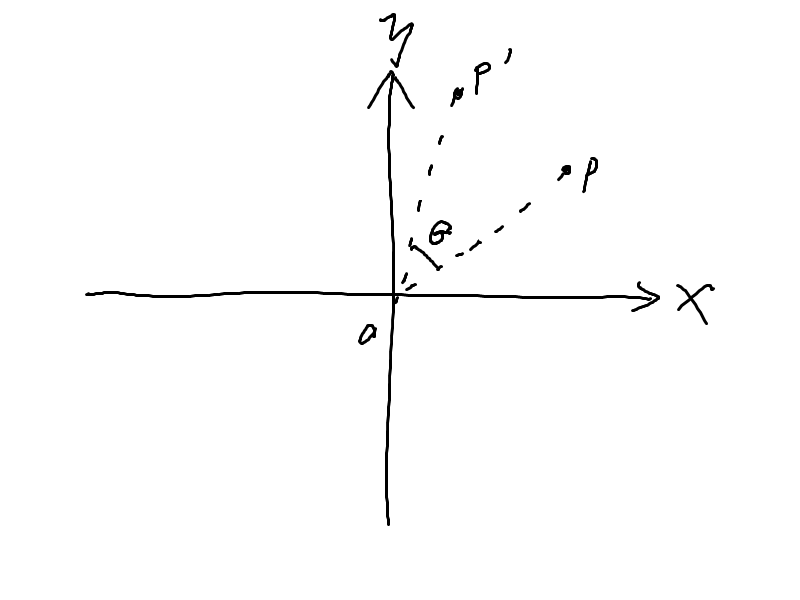
\includegraphics[width=0.33\linewidth]{fig/rotate.png}
\caption{把$OP$转过去}
\label{fig-rotate}
\end{figure}

如果用矢量$\mathbf{P}=\begin{bmatrix} x_p \\ y_p \end{bmatrix}$表示$P$的坐标,矩阵$\mathbf{R}(\theta)=\begin{bmatrix}
\cos \theta & -\sin \theta \\
\sin \theta & \cos \theta
\end{bmatrix}$表示旋转操作(它的元素是$\theta$的函数),那么$P$的坐标$\mathbf{P'}=\mathbf{R}(\theta) \mathbf{P}$,这样看起来就比较厉害。

【练习】证明$\mathbf{R}(\alpha) \mathbf{R}(\beta)=\mathbf{R}(\alpha+\beta)$。

矩阵不但可以表示旋转,还可以表示缩放。比如$\mathbf{S}=\begin{bmatrix}
2 & 0 \\
0 & 1
\end{bmatrix}$就表示把$x$坐标放大到原来的$2$倍,而$y$坐标不变。

如果把$P$旋转$\theta$角,再把$x$坐标放大到$2$倍,然后旋转$\phi$角得到$P'$,只要依次把矩阵从右到左乘起来就行了,也就是$\mathbf{P'}=\mathbf{R}(\phi) \mathbf{S} \mathbf{R}(\theta) \mathbf{P}$。这样就能直观地看出矩阵乘法不满足交换律。(从右到左写的习惯和我们熟悉的函数一样,比如$f_2(f_1(x))$表示对$x$先进行$f_1$这个操作,再进行$f_2$这个操作)

日常生活中有许多东西不满足交换律,比如你爸爸的妈妈和你妈妈的爸爸不是同一个人,再比如三维空间中先向左转$90$度,再向上转$90$度与先向上转$90$度,再向左转$90$度是不一样的。这样的东西在数学上称为\emph{非阿贝尔群}。

【练习】$\mathbf{A}=\begin{bmatrix}
0 & 1 & 0 & 0 \\
1 & 0 & 0 & 0 \\
0 & 0 & 1 & 0 \\
0 & 0 & 0 & 1
\end{bmatrix}$,$\mathbf{B}=\begin{bmatrix}
1 & 2 & 3 & 4 \\
5 & 6 & 7 & 8 \\
9 & 10 & 11 & 12 \\
13 & 14 & 15 & 16
\end{bmatrix}$,求$\mathbf{A} \mathbf{B}$和$\mathbf{B} \mathbf{A}$。$\mathbf{A}$乘在左边和右边分别表示什么操作?

在计算矩阵乘法时经常出现求和号。有一天爱因斯坦说:两个矩阵相乘,如果有相同的下标就表示求和,求和号可以不写。比如$C_{i k}=\sum_j A_{i j} B_{j k}$可以写成$C_{i k}=A_{i j} B_{j k}$,而$\mathbf{P'}=\mathbf{R}(\phi) \mathbf{S} \mathbf{R}(\theta) \mathbf{P}$可以写成$P'_i=R_{i j}(\phi) S_{j k} R_{k l}(\theta) P_l$。如果没有相同的指标就不表示求和,比如$A_i$是一个$m$列的矢量,$B_i$是一个$n$列的矢量,$C_{i j}=A_i B_j$,那么$C_{i j}$就是一个$m$行$n$列的矩阵。

(用什么字母作为下标不会影响矩阵的内容,比如$A_{i j}$和$A_{k l}$表示的是同一个矩阵)
\section{对矩阵求导}
在平面上的一个静止的参考系$S$中,有一个矢量$\mathbf{A}$,它可以随着时间变化。在以角速度$\omega$顺时针旋转的参考系$S'$中看,得到$\mathbf{A'}=\mathbf{R} \mathbf{A}$,其中$\mathbf{R}=\begin{bmatrix}
\cos \omega t & -\sin \omega t \\
\sin \omega t & \cos \omega t
\end{bmatrix}$,它也是时间$t$的函数。

现在来看$S'$系中$\mathbf{A'}$的速度:$\frac{\opd \mathbf{A'}}{\opd t}=\frac{\opd \mathbf{R}}{\opd t} \mathbf{A}+\mathbf{R} \frac{\opd \mathbf{A}}{\opd t}$。

对两个矩阵的乘积求导,跟对两个数的乘积求导是一样的,因为计算导数的时候没有用到乘法交换律。容易理解,$\mathbf{R} \frac{\opd \mathbf{A}}{\opd t}$就是把$S$系中$\mathbf{A}$的速度用$\mathbf{R}$旋转一下。但是$\frac{\opd \mathbf{R}}{\opd t} \mathbf{A}$是什么意思呢?

我们直接计算$\frac{\opd \mathbf{R}}{\opd t}=\begin{bmatrix}
-\sin \omega & -\cos \omega \\
\cos \omega & -\sin \omega
\end{bmatrix}$,也就是对矩阵中的每个元素分别求导。然后计算$\frac{\opd \mathbf{R}}{\opd t} \mathbf{A}$就会发现,它是一个矢量,大小为$\omega A$,方向为$\mathbf{A}$逆时针转$90$度,相当于旋转引起的线速度。

也可以用直观的几何方法来理解,如图\ref{fig-rotate-deri},$\frac{\opd \mathbf{R}}{\opd t} \mathbf{A}=\frac{1}{\opd t}(\mathbf{R}(t+\opd t) \mathbf{A}-\mathbf{R}(t) \mathbf{A})$,当$\opd t$无限小时,它的方向垂直于$\mathbf{A}$。
\begin{figure}[htb]
\centering
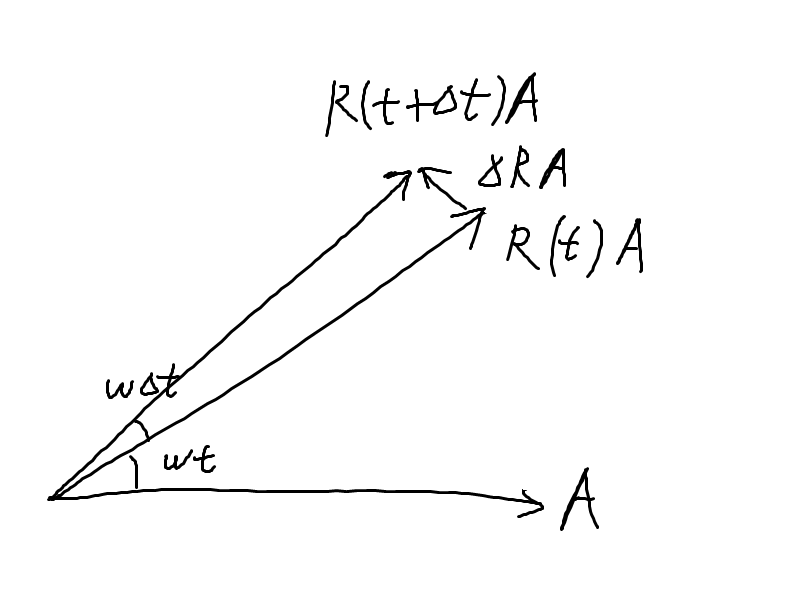
\includegraphics[width=0.33\linewidth]{fig/rotate-deri.png}
\caption{把$\mathbf{A}$转过去}
\label{fig-rotate-deri}
\end{figure}

(用类似的方法可以求$A'$的加速度,但是理解起来比较麻烦,以后再讲)
\section{零矩阵;单位矩阵;逆矩阵}
零矩阵$\mathbf{0}$就是$\begin{bmatrix}
0 & 0 & \dots & 0 \\
0 & 0 & \dots & 0 \\
\vdots & \vdots & \ddots & \vdots \\
0 & 0 & \dots & 0
\end{bmatrix}$这样的矩阵。它的行数与列数是多少可以根据上下文判断。一个矩阵跟(大小合适的)$\mathbf{0}$相加,得到的矩阵与原来一样;跟$\mathbf{0}$相乘(不管在左边还是右边),得到$\mathbf{0}$。

单位矩阵$\mathbf{I}$就是$\begin{bmatrix}
1 & 0 & \dots & 0 \\
0 & 1 & \dots & 0 \\
\vdots & \vdots & \ddots & \vdots \\
0 & 0 & \dots & 1
\end{bmatrix}$这样的矩阵。一般认为它的行数与列数相同,具体是多少也要根据上下文判断。一个矩阵跟$\mathbf{I}$相乘,得到的矩阵与原来一样。

如果两个矩阵$\mathbf{A}$和$\mathbf{A'}$相乘得到$\mathbf{I}$,那么$\mathbf{A}$和$\mathbf{A'}$互为逆矩阵。如果$\mathbf{A'} \mathbf{B}=\mathbf{C}$,那么在$\mathbf{C}$前面再乘一个$\mathbf{A}$又得到了$\mathbf{B}$(别忘了矩阵乘法满足结合律),就像是除以$\mathbf{A'}$一样。

然而不是每个矩阵都存在逆矩阵,即使逆矩阵存在,从$\mathbf{A}$算出$\mathbf{A'}$也比较麻烦。一种容易理解但是不容易算的方法是待定系数法,更好的方法需要利用行列式的性质,我们以后再讲。逆矩阵有许多实际应用,在各种实际情况下快速计算逆矩阵是一个热门的问题。

【练习】证明$\begin{bmatrix}
1 & 2 \\
3 & 4
\end{bmatrix}$的逆矩阵是$\begin{bmatrix}
-2 & 1 \\
\frac{3}{2} & -\frac{1}{2}
\end{bmatrix}$。
\section{行列式;坐标系的手性}
行数和列数相同的矩阵叫作方阵,它的行数或者列数也可以叫作阶数。行列式是一个把方阵变成实数的操作,矩阵$\mathbf{A}$的行列式用$\det \mathbf{A}$或者$|\mathbf{A}|$表示。(行列式的绝对值用$||\mathbf{A}||$表示)

二阶行列式$\begin{vmatrix}
a & b \\
c & d
\end{vmatrix}=a d-b c$,三阶行列式$\begin{vmatrix}
a & b & c \\
d & e & f \\
g & h & i
\end{vmatrix}=a e i+b f g+c d h-c e g-a f h-b d i$(找一找这个式子的规律)。更高阶的行列式计算比较麻烦,而且不常用,我们待会再讲。

这个东西有什么用呢?在二维平面内,如果点$P(x_P, y_P), Q(x_Q, y_Q)$,那么$S_{\triangle O P Q}=\frac{1}{2}\begin{vmatrix}
x_P & y_P \\
x_Q & y_Q
\end{vmatrix}$。你可以用解析几何验证一下。这就是传说中的叉积$\mathbf{P} \times \mathbf{Q}$的二维形式。

(顺便说一句,二维矢量的叉积是一个标量,三维矢量的叉积是一个矢量,更高维度的叉积以后再讲。)

这个“面积”算出来有可能是负的,因为$P$和$Q$在行列式中的位置不一样。可以用右手螺旋来判断:把右手四指指向$O P$方向,然后转向$O Q$方向。如果大拇指朝上,那么就是正的,否则就是负的。高考范围内一般只要取绝对值就行了。算三角形面积别忘了乘$\frac{1}{2}$。

在三维空间内,如果点$P(x_P, y_P, z_P), Q(x_Q, y_Q, z_Q), R(x_R, y_R, z_R)$,那么三棱锥$O-P Q R$的体积$V=\frac{1}{6}\begin{vmatrix}
x_P & y_P & z_P \\
x_Q & y_Q & z_Q \\
x_R & y_R & z_R
\end{vmatrix}$。这样可以秒杀一些立体几何题。这个“体积”也有可能是负的,记得取绝对值。

如果把矩阵看作一个坐标变换,那么行列式就是坐标变换之后和之前的图形的体积(不管几维都叫体积好了)之比。比如二维情况下,设矩阵$\mathbf{A}=\begin{bmatrix}
a & b \\
c & d
\end{bmatrix}$是一个坐标变换,点$\mathbf{P}=\begin{bmatrix} 1 \\ 0 \end{bmatrix}$,$\mathbf{Q}=\begin{bmatrix} 0 \\ 1 \end{bmatrix}$,$\mathbf{P'}=\mathbf{A} \mathbf{P}=\begin{bmatrix} a \\ c \end{bmatrix}$(这里不严格区分点和它对应的矢量),$\mathbf{Q'}=\mathbf{A} \mathbf{Q}=\begin{bmatrix} b \\ d \end{bmatrix}$,那么$S_{\triangle O P Q}=\frac{1}{2}(a d-b c)$。只要对单位三角形$\triangle O P Q$验证了这一点,由面积的可加性,这一点对任意图形都是成立的。

如果这个“体积”之比是负的,说明这个坐标变换改变了坐标系的\emph{手性}。不管在几维空间内,都存在着两种手性的坐标系,我们一般习惯用右手系。比如二维情况下,坐标变换$\begin{bmatrix}
-1 & 0 \\
0 & 1
\end{bmatrix}$把$x$轴反过来(专业一点叫\emph{空间反演变换}),$y$轴不变,那么坐标系的手性就改变了。同时反转$x$轴和$y$轴不会改变坐标系的手性,旋转变换也不会。

如果$\mathbf{A}$是$n$维矩阵,$c$是实数,那么$|c \mathbf{A}|=c^n |\mathbf{A}|$。矩阵乘法可以表示两次连续的坐标变换,所以$|\mathbf{A} \mathbf{B}|=|\mathbf{A}| |\mathbf{B}|$。如果方阵的一行或者一列全是$0$,那么行列式就是$0$。

行列式只是一种数学工具,图形的体积和变换的体积之比是它的两种应用,在其他地方还会遇到类似的式子。
\section{用行列式解线性方程组}
现在用看起来很厉害的方法解二元一次方程组
\begin{equation*}
\begin{cases}
a_{1 1} x_1+a_{1 2} x_2=b_1 \\
a_{2 1} x_1+a_{2 2} x_2=b_2 \\
\end{cases}
\end{equation*}

如果$b_1, b_2$不全为$0$,先设$D=\begin{vmatrix}
a_{1 1} & a_{1 2} \\
a_{2 1} & a_{2 2}
\end{vmatrix}$。如果$D \neq 0$,我们说这两个方程线性无关(也就是独立),可以解出$x_1=\frac{1}{D}\begin{vmatrix}
a_{1 1} & b_1 \\
a_{2 1} & b_2
\end{vmatrix}$,$x_2=\frac{1}{D}\begin{vmatrix}
a_{1 2} & b_1 \\
a_{2 2} & b_2
\end{vmatrix}$。你可以用消元法暴算出方程的解,然后比较一下。如果两种方法都很熟悉,运算量是差不多的。

如果$D=0$,说明方程组无解或者有无穷多个解,具体是哪种情况要解解看才知道。我们说这两个方程线性相关,也就是说它们乘一个倍数可以变成同一个方程。

如果$b_1=b_2=0$,也就是说这是一个齐次方程组。如果$D \neq 0$,用上面的方法算出$x_1=x_2=0$,这确实是一个解,但是没有非零解,也就是说矢量$(a_{1 1}, a_{2 1})$和$(a_{1 2}, a_{2 2})$不共线。如果$D=0$,有无穷多个解。

类似的方法可以解三元或者更多元的线性方程组,以及判断三维空间中矢量的共面情况。这些事情的严格证明一般是先证明二阶的情况,再用归纳法证明更高阶的情况。
\section{高阶行列式}
(这部分内容看不懂可以先跳过,有兴趣的同学可以去看线性代数的书)

首先定义$P_i$是自然数$1, 2, 3, \dots, n$的一个排列,称为$n$阶排列。比如$(2, 1, 3, 4, 5), (5, 4, 3, 2, 1)$都是$5$阶排列。不同的下标$i$表示不同的排列,而不是排列中的第$i$个元素。

然后定义一个操作叫置换,就是把排列里的两个数换一下。比如$5$阶排列$(1, 2, 3, 4, 5)$经过置换可以得到$(2, 1, 3, 4, 5)$,再置换一次可以得到$(2, 3, 1, 4, 5)$等等。任何一个$n$阶排列都可以从$(1, 2, 3, \dots, n)$经过置换得到。

我们要把所有排列分成两类:奇排列和偶排列。设$(1, 2, 3, \dots, n)$至少经过$m$次置换才能得到$P_i$,如果$m$是奇数,$P_i$就是奇排列,否则是偶排列。

接着定义一个正负号函数$sgn(P_i)$:如果$P_i$是奇排列,那么$sgn(P_i)=+1$,否则$sgn(P_i)=-1$。

现在可以定义$n$阶方阵$\mathbf{A}$的行列式
\begin{equation*}
|\mathbf{A}|=\sum_{P_i} sgn(P_i) \prod_{k=1}^n A_{k P_k}
\end{equation*}

其中求和是对所有$n$阶排列$P_i$求和,$\prod$表示连乘。比如$n=5$时,共有$120$个排列,其中有一个是$P_i=(2, 3, 1, 4, 5)$,它是偶排列,那么求和号里就有一项$-A_{1 2} A_{2 3} A_{3 1} A_{4 4} A_{5 5}$。把$120$项加起来就得到了行列式的值。你可以验证一下前面说的二阶和三阶行列式符合这样的定义。

这是行列式的一种定义,但是真的用这种方法计算是很麻烦的。$n$阶排列共有$n!$个,所以这种方法的复杂度是$O(n!)$。我们已经知道可以用行列式解线性方程组,而解线性方程组有$O(n^3)$的方法,那么算行列式肯定也有$O(n^3)$的方法,称为\emph{高斯消元法}。行列式还有许多运算技巧,我们以后再讲。
\section{矩阵的幂;矩阵级数}
定义了矩阵乘法之后就可以定义幂运算。比如$\mathbf{A}^2=\mathbf{A} \mathbf{A}$。但是矩阵的幂运算并不常用,只有矩阵是方阵,并且指数是整数的时候才有意义。矩阵乘法不满足交换律,所以$(\mathbf{A} \mathbf{B})^2=\mathbf{A}^2 \mathbf{B}^2$这样的公式也不成立。

如果把一个函数表示成级数,它的定义域和值域可以都是矩阵。比如
\begin{equation*}
\rme^\mathbf{A}=\sum_{n=0}^{\infty}\frac{1}{n!}\mathbf{A}^n=1+\mathbf{A}+\frac{1}{2}\mathbf{A}^2+\frac{1}{6}\mathbf{A}^3+\dots
\end{equation*}

这样一来,线性微分方程组
\begin{align*}
\opdt x_1 &=a_{1 1} x_1+a_{1 2} x_2+\dots+a_{1 n} x_n \\
\opdt x_2 &=a_{2 1} x_1+a_{2 2} x_2+\dots+a_{2 n} x_n \\
&\dots \\
\opdt x_2 &=a_{n 1} x_1+a_{n 2} x_2+\dots+a_{n n} x_n
\end{align*}

可以直接写成$\opdt \mathbf{x}=\mathbf{a} \mathbf{x}$,它的解就是$\mathbf{x}=\rme^{t \mathbf{a}} \mathbf{x_0}$。(注意字母相乘的顺序,解微分方程的时候并没有用到乘法交换律)

$\mathbf{x_0}$表示初始条件,而$\rme^{t \mathbf{a}}$表示系统随着时间演化的规律。不管初始条件是什么,演化的规律总是相同的。然而要计算出矩阵函数的值,并不是一件容易的事情。
\section{线性空间}
实数、复数、矢量和矩阵有一些共同点,比如都能进行加法和数乘运算,这样的集合叫作线性空间。

严格来说,线性空间的定义是这样的:设$V$是一个集合,$a, b, c$是它的元素,$\lambda, \mu$是数。定义一种加法运算把两个元素变成一个元素,数乘运算把一个数和一个元素变成一个元素,它们满足:
\begin{enumerate}
\item $(a+b)+c=a+(b+c)$。
\item $a+b=b+a$。
\item 存在一个元素$0$,对任何元素$a$,$a+0=a$。(其实这句话中的“一个”不是必须的)
\item 对任何元素$a$,存在一个元素$-a$,$a+(-a)=0$。
\item $1 a=a$。
\item $(\lambda \mu) a=\lambda (\mu a)$。
\item $(\lambda+\mu) a=\lambda a +\mu a$。
\item $\lambda (a+b)=\lambda a +\lambda b$。
\end{enumerate}

(更抽象的定义中$\lambda$不一定是数,可以是其他奇怪的东西,关于数域的事情以后再讲。)

实数集$R$和复数集$C$都是线性空间。行数为$m$,列数为$n$的所有矩阵组成的集合$M(m, n)$也是线性空间。如果一个公式里只出现加法和数乘运算,那么不管里面的字母属于什么线性空间,都可以把公式套上去用。比如$F=m a$中的$F$和$a$有时候理解成实数,有时候理解成矢量。

以后讲量子力学的时候会用到这些东西,讲傅立叶变换的时候还会用到。
